%% ============================================================================
%% Capítulo 1 — Introdução
%%
%% Fontes da verdade (todo número rastreia aos capítulos já escritos):
%%   - cap5-benchmark.tex ..... empate 8/10 ROPE; eta^2=0,20; TabFM 2,7/1,0/1,2
%%     e 13/18; latências 43.262 vs 0,33 us/linha (131.097x); KANs último terço
%%   - cap6-framework.tex ..... LODO 0,11 vs 0,44 (@11) e 0,72 vs 0,78 (@14);
%%     sempre-FM regret médio 0,021 / mediano 0,000; E2 cruzamento entre
%%     w=0,9 e w=0,8 (10-20% de peso na latência)
%%   - cap7-destilacao.tex .... pontual 4/20; distribucional 16/20, mediana
%%     +0,19, sinal p=0,006; fronteira 2,5x/27x; OOF 0,5-5,1 p.p. PICP80;
%%     E1 17/20, p=0,0013
%%   - cap4-metodologia.tex ... 14x18, 250/252, protocolo
%% Estrutura: blueprint (docs/blueprint-dissertacao.md) + guia didático
%% (docs/guia-escrita-didatica.md). Sem caixa-resumo neste capítulo (seria
%% redundante com o resumo pré-textual).
%%

\chapter{Introdução}
\label{chap:introducao}

\section{Contexto e motivação}
\label{sec:intro-contexto}

``Em dados tabulares, \emph{gradient boosting} sempre vence.'' Poucas
máximas da prática de aprendizado de máquina foram tão repetidas na última
década --- e, ao contrário da maioria, esta chegou a receber forma
quantitativa: em 2022, um estudo sistemático identificou os vieses
indutivos que explicam por que comitês de árvores superam redes neurais em
tabelas típicas \citep{grinsztajn2022}, e avaliações subsequentes em escala
maior matizaram, sem derrubar, o veredito \citep{mcelfresh2023}. Para o
praticante, a máxima virou atalho de decisão: diante de uma tabela, use
XGBoost e siga em frente.

Considere, porém, a decisão concreta que essa máxima pretende resolver. Um
time de ciência de dados precisa escolher o modelo que decidirá, em
produção, aprovações de crédito --- um problema da família dos conjuntos
\texttt{credit\_g} e \texttt{give\_me\_some\_credit} deste estudo --- ou o
que estimará preços de imóveis com intervalos de confiança, como no
\texttt{california\_housing}. Em 2026, esse time encontra um cardápio que a
máxima não previa: além dos três \emph{gradient boostings} consolidados,
há uma dúzia de arquiteturas profundas que alegam tê-los alcançado, duas
redes de Kolmogorov--Arnold com alegações fortes de superioridade e, no
centro das atenções, os \emph{foundation models} tabulares --- redes
pré-treinadas que dispensam qualquer treinamento na tarefa: o conjunto de
treino entra como contexto no momento da predição
\citep{hollmann2025,tabfm2026}. Cada proponente publica números a seu
favor, medidos sob protocolos distintos, com orçamentos de ajuste
distintos e, com frequência crescente, sem revisão por pares. O que falta
ao time não é mais um modelo: é evidência neutra, produzida sob um
protocolo único, e um procedimento defensável para converter essa
evidência em escolha.

Esta dissertação produz as duas coisas --- e o retrato que emerge dela
justifica o esforço, porque contraria a máxima duas vezes. Primeiro, na
geração de modelos anterior a 2026, o topo da acurácia é um \emph{empate
estatístico}: sob região de equivalência prática de um ponto percentual de
AUC, 8 dos 10 modelos não-líderes são praticamente equivalentes ao líder,
e 80\% da variância de desempenho está \emph{dentro} das famílias, não
entre elas --- ``\emph{boosting} sempre vence'' não encontra margem de
acurácia que a sustente (Capítulo~\ref{chap:benchmark}). Segundo, a
geração 2026 quebra o empate em direção inesperada: não foi o aprendizado
profundo ajustado que alcançou as árvores, foi o pré-treino que atropelou
ambos --- o TabFM, avaliado \emph{zero-shot}, sem qualquer ajuste, é o
melhor modelo em \textbf{13 dos 18 conjuntos} do benchmark e lidera o rank
médio nas três tarefas. O preço, contudo, muda a natureza da decisão: o
líder de acurácia custa cerca de \textbf{43 milissegundos por linha} para
servir predições, contra \textbf{0,33 microssegundos} do XGBoost ---
quatro a cinco ordens de magnitude, um fator de aproximadamente 131~mil
vezes no conjunto de referência. A pergunta prática deixou de ser ``qual
família vence?'' e passou a ser ``a latência do líder cabe no meu caso de
uso --- e, se não cabe, o que fazer?''.

É essa segunda pergunta que dá à dissertação sua terceira frente. Se o
obstáculo à adoção do líder é um custo de arquitetura --- o conjunto de
treino que viaja com o modelo a cada predição ---, custos de arquitetura
podem, em princípio, ser transferidos: a destilação de conhecimento
\citep{hinton2015} treina um aluno de microssegundos nas saídas do
professor caro. Para \emph{foundation models} tabulares, a literatura
estabeleceu essa rota em classificação \citep{pocketfm2026}; o que ela
transfere em \emph{regressão} --- em particular quando o que se quer
preservar não é um número, mas a distribuição preditiva completa, com
quantis e intervalos calibrados --- permanecia, até as verificações
datadas deste estudo, sem resposta pública. A resposta que encontramos é
seletiva e, por isso mesmo, útil: a destilação \emph{pontual} falha de
forma robusta, a destilação \emph{distribucional} funciona onde o
professor tem vantagem genuína, e a fronteira entre as duas condições é
verificável em minutos (Capítulo~\ref{chap:destilacao}).

\section{Problema de pesquisa}
\label{sec:intro-problema}

O problema que esta dissertação enfrenta pode ser enunciado em três
camadas, cada uma herdando a anterior. Na primeira camada, há um
\emph{vácuo de evidência comparável}: as famílias de modelos tabulares
disponíveis em 2026 --- \emph{gradient boosting}, aprendizado profundo em
suas três linhagens e \emph{foundation models} de aprendizado em contexto
--- não haviam sido medidas sob um protocolo único que combinasse
validação honesta (seleção de hiperparâmetros estritamente separada da
medição), inferência estatística capaz de \emph{afirmar} equivalências
além de rejeitá-las, e eixos de custo --- tempo de treino, custo de ajuste
e latência de serviço --- medidos nas mesmas condições que a acurácia. Os
benchmarks de referência são anteriores à geração 2026
\citep{grinsztajn2022,mcelfresh2023}, e os números dessa geração provinham
majoritariamente dos próprios proponentes.

Na segunda camada, mesmo com a evidência produzida, resta o problema da
\emph{decisão}: benchmarks descrevem, mas times precisam escolher. A
literatura de seleção de algoritmos sugere aprender um roteador a partir
de meta-características do problema \citep{rice1976}; a honestidade exige
testar se tal roteador generaliza no regime real --- poucas dezenas de
conjuntos de dados --- antes de recomendá-lo, e a literatura raramente
reporta esse teste. Um artefato de decisão que nunca foi validado contra
dados que não participaram de sua construção é uma hipótese, não um
instrumento.

Na terceira camada, a evidência e o artefato de decisão apontam juntos
para um único obstáculo operacional: a latência do novo líder de acurácia.
O problema torna-se, então, de engenharia dirigida por ciência: determinar
o que a destilação de conhecimento pode e não pode transferir de um
\emph{foundation model} tabular em regressão, a que custo de serviço, e
sob quais condições verificáveis \emph{a priori} --- com a regressão
distribucional, eixo em que o professor carrega informação que os dados
brutos não entregam ao aluno, como recorte central.

\section{Objetivos}
\label{sec:intro-objetivos}

\subsection{Objetivo geral}

Estabelecer, sob protocolo experimental único
e estatisticamente honesto, a evidência comparativa das três famílias de
modelos tabulares na era dos \emph{foundation models}, e convertê-la em
instrumentos validados de decisão --- incluindo a avaliação, por
destilação de conhecimento, de até que ponto o principal obstáculo
operacional da família líder pode ser removido.

\subsection{Objetivos específicos}

\begin{itemize}
  \item Executar um benchmark multicritério de 14 modelos sobre 18
    conjuntos de dados públicos do OpenML, sob validação cruzada aninhada
    com \emph{hold-out} intocado, orçamentos de ajuste equalizados por
    custo e inferência estatística frequentista \emph{e} bayesiana com
    região de equivalência prática;
  \item Medir, sob o mesmo protocolo, os eixos de custo que a literatura
    raramente reporta --- tempo de treino, custo total de ajuste de
    hiperparâmetros e latência de inferência --- e cruzá-los com o
    desempenho em fronteiras de Pareto;
  \item Incluir e adjudicar, com verificação de novidade datada, as duas
    adições de 2026: a comparação neutra entre os dois \emph{foundation
    models} (TabPFN e TabFM) e o primeiro teste independente da família
    Kolmogorov--Arnold contra a grade completa de famílias;
  \item Construir um arcabouço de decisão orientado a restrições e
    validá-lo por \emph{leave-one-dataset-out}, confrontando o roteamento
    aprendido por meta-características com políticas fixas sob métrica de
    \emph{regret} --- incluindo a extensão pré-registrada ao \emph{regret}
    multicritério ponderado por preferências de latência;
  \item Investigar o que a destilação de conhecimento transfere de
    \emph{foundation models} tabulares em regressão --- pontual e
    distribucional ---, medir a fronteira de estratégias de serviço
    (destilar, comprimir contexto, reduzir \emph{ensemble}) nos mesmos
    \emph{hold-outs}, testar o aluno destilado contra \emph{baselines}
    distribucionais clássicos em experimento pré-registrado, e condensar
    as condições de valor numa regra de decisão prática;
  \item Sustentar todas as conclusões em infraestrutura reprodutível ---
    sementes, versões e dados fixados, artefatos versionados --- sob um
    contrato explícito de conduta científica (pré-registro de hipóteses,
    verificação datada de novidade, reporte de resultados negativos e
    correção por retificação).
\end{itemize}

\section{Perguntas de pesquisa}
\label{sec:intro-qps}

Três perguntas de pesquisa organizam a dissertação; cada uma é respondida
por um capítulo de resultados, e as três são retomadas, com a evidência
acumulada, na conclusão.

\begin{description}
  \item[QP1.] \emph{O empate de acurácia entre as famílias de modelos
    tabulares sobrevive a um protocolo rigoroso --- validação aninhada,
    equivalência prática bayesiana, eixos de custo --- e à chegada da
    geração 2026 de foundation models?}
    (Capítulo~\ref{chap:benchmark})
  \item[QP2.] \emph{Que artefato de decisão um benchmark com $N$ realista
    de conjuntos consegue, honestamente, sustentar --- um roteador
    aprendido ou uma política por restrições --- e como essa resposta
    muda quando a decisão pondera acurácia e custo?}
    (Capítulo~\ref{chap:framework})
  \item[QP3.] \emph{O que a destilação de conhecimento transfere de um
    foundation model tabular em regressão, a que custo de serviço, e sob
    quais condições verificáveis a priori?}
    (Capítulo~\ref{chap:destilacao})
\end{description}

A Figura~\ref{fig:intro-qps} resume o encadeamento: a resposta de cada
pergunta cria a pergunta seguinte --- o empate e sua quebra (QP1) tornam a
decisão multicritério inevitável (QP2), e a política de decisão validada
esbarra num único obstáculo, cuja remoção é o objeto da QP3. No diagrama,
as setas sólidas ligam cada pergunta ao capítulo que a responde, e as
tracejadas marcam esse encadeamento lógico; os
Capítulos~\ref{chap:fundamentacao} a~\ref{chap:metodologia} fornecem,
respectivamente, o vocabulário, o posicionamento na literatura e o
protocolo comuns às três frentes.

\begin{figure}[htb]
\centering
% Diagrama pré-compilado (fonte editável: tikz-src/tikz-cap1-1.tex;
% recompilar com: tectonic tikz-src/tikz-cap1-1.tex && mv tikz-cap1-1.pdf images/)
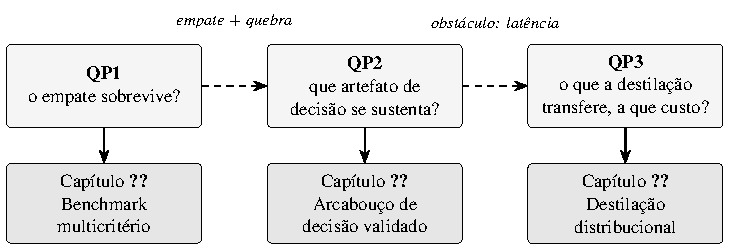
\includegraphics{images/tikz-cap1-1.pdf}
\caption{Perguntas de pesquisa e capítulos que as respondem.}
\label{fig:intro-qps}
\end{figure}

\section{Resumo das contribuições}
\label{sec:intro-contribuicoes}

As contribuições desta dissertação são de \emph{medição sob protocolo
uniforme} e de \emph{validação honesta} --- não se reivindica mecanismo
novo de aprendizado; reivindica-se, com verificações de novidade datadas,
o recorte e a evidência que faltavam. Em ordem de apresentação:

\begin{enumerate}
  \item \textbf{Um benchmark multicritério da era dos foundation models}
    --- 14 modelos $\times$ 18 conjuntos (250 das 252 células; duas
    exclusões estruturais declaradas), com validação cruzada aninhada,
    inferência frequentista e bayesiana e três eixos de custo sob o mesmo
    protocolo. Dele saem os dois fatos que estruturam a dissertação: o
    empate estatístico da geração anterior (8 de 10 modelos praticamente
    equivalentes ao líder; 80\% da variância de rank intrafamília) e a
    quebra do empate pela geração 2026 (TabFM líder nas três tarefas e
    melhor modelo em 13 de 18 conjuntos, \emph{zero-shot}, ao preço de
    quatro a cinco ordens de magnitude em latência). Inclui a primeira
    comparação neutra TabPFN~$\times$~TabFM sob protocolo idêntico, até
    onde alcançam as verificações datadas (Capítulo~\ref{chap:benchmark}).
  \item \textbf{Um resultado negativo independente sobre as redes de
    Kolmogorov--Arnold} --- no primeiro teste da família contra a grade
    completa GBDT/aprendizado profundo/\emph{foundation models} em
    benchmark multicritério (verificação datada), KAN e TabKAN terminam no
    último terço nas três tarefas, embora baratas de servir: sob protocolo
    uniforme com ajuste equalizado, as alegações dos artigos originais não
    se sustentam (Capítulo~\ref{chap:benchmark}).
  \item \textbf{Um arcabouço de decisão validado, não apenas descrito} ---
    três estudos sob \emph{leave-one-dataset-out} elevam o fluxograma de
    decisão de descritivo a validado: o roteamento por meta-características
    não generaliza (taxa de acerto 0,11 contra 0,44 do \emph{baseline}
    trivial no estudo com 11 modelos; 0,72 contra 0,78 com 14); a política
    fixa ``\emph{foundation model} primeiro'' é \emph{regret}-ótima na
    métrica primária, com \emph{regret} mediano zero na geração 2026; e o
    experimento pré-registrado E2, contribuição exclusiva desta
    dissertação, localiza o ponto de inversão --- basta deslocar 10 a 20\%
    do peso da acurácia para a latência para a recomendação virar ---,
    justificando quantitativamente a arquitetura do fluxograma
    (Capítulo~\ref{chap:framework}).
  \item \textbf{A destilação distribucional de foundation models
    tabulares} --- o recorte verificado como inédito: sob desenho
    pré-registrado em 20 conjuntos, a destilação \emph{pontual} falha de
    forma robusta com qualquer professor (um resultado negativo reportado
    com proeminência integral), enquanto a transferência das curvas de
    quantis retém mediana de 19\% da vantagem distribucional do professor,
    positiva em 16 de 20 conjuntos (teste de sinal $p=0{,}006$), a
    latências de microssegundos; a primeira fronteira medida de ponta a
    ponta entre destilar, comprimir contexto e reduzir \emph{ensemble}; a
    ablação que mostra que a rotulagem \emph{out-of-fold} protege
    calibração, não acurácia; o experimento pré-registrado E1, também
    exclusivo desta dissertação, em que o aluno destilado vence
    \emph{baselines} distribucionais clássicos em 17 de 20 conjuntos
    ($p=0{,}0013$); e a regra de decisão prática que converte as
    refutações em instrução verificável em minutos
    (Capítulo~\ref{chap:destilacao}).
  \item \textbf{Infraestrutura e conduta reutilizáveis} --- o protocolo, os
    artefatos versionados (cada número do texto rastreia a um CSV,
    JSON ou notebook executado), os pré-registros com adendos datados, as
    verificações de novidade registradas e o rito de errata pública
    constituem, em conjunto, uma contribuição metodológica de
    reprodutibilidade, descrita no Capítulo~\ref{chap:metodologia} e
    exercitada ao longo de toda a parte empírica.
\end{enumerate}

\section{Produção bibliográfica}
\label{sec:intro-producao}

A pesquisa gerou, até o depósito desta dissertação, dois relatórios
técnicos do programa de pós-graduação, correspondentes às disciplinas de
trabalho individual, ambos em inglês e disponíveis no repositório público
do projeto:

\begin{itemize}
  \item \textbf{AI-1} --- \emph{Does ``GBDT Always Win''? A Multi-Criteria
    Benchmark of 14 Tabular Models --- From a Statistical Tie to the 2026
    Break --- and a Validated Decision Framework} \citep{companion2026}:
    relatório técnico do Trabalho Individual (\texttt{latex/ai1/} no
    repositório), que condensa o material dos
    Capítulos~\ref{chap:benchmark} e~\ref{chap:framework}.
  \item \textbf{AI-2} --- \emph{Distilling Tabular Foundation Models
    Beyond Classification: Distributional Regression and the
    Distill/Compress/Shrink Pareto Frontier} \citep{companion-ai2-2026}: relatório técnico da Atividade de
    Orientação Individual (\texttt{latex/ai2/}), que condensa o material
    do Capítulo~\ref{chap:destilacao}; um preprint derivado dele está em
    preparação para submissão ao arXiv.
\end{itemize}

Os dois relatórios são trabalhos avaliativos do programa, sem revisão por
pares externa até a data desta escrita; seu conteúdo corresponde,
respectivamente, aos Capítulos~\ref{chap:benchmark}
e~\ref{chap:framework} e ao Capítulo~\ref{chap:destilacao}, que incluem
ainda os dois experimentos (E1 e E2) que são contribuições novas da
dissertação, inéditas em relação aos relatórios.

\section{Como ler esta dissertação}
\label{sec:intro-comoler}

A dissertação foi escrita para três perfis de leitor, e nem todos precisam
percorrê-la linearmente. O \textbf{praticante} --- quem precisa escolher e
servir um modelo tabular --- pode ir diretamente aos
Capítulos~\ref{chap:benchmark} e~\ref{chap:framework} (a evidência e o
fluxograma de decisão) e à regra de decisão que encerra o
Capítulo~\ref{chap:destilacao} (Seção~\ref{sec:destil-regra}): os três
pontos foram escritos para serem autocontidos, com os pré-requisitos
mínimos recapitulados no início de cada capítulo. O \textbf{leitor de
formação estatística} interessado no rigor das comparações deve começar
pela Seção~\ref{sec:fund-estatistica} do Capítulo~\ref{chap:fundamentacao}
(a teoria dos testes, incluindo a camada bayesiana de equivalência
prática) e pelo Capítulo~\ref{chap:metodologia} (o protocolo de aplicação,
a política para células faltantes e as limitações declaradas antes dos
resultados). O \textbf{replicador} --- quem quer reproduzir ou estender os
experimentos --- encontra no Capítulo~\ref{chap:metodologia} o protocolo
completo com sementes, versões e justificativas, e nos apêndices o
restante: as tabelas completas por conjunto
(Apêndice~\ref{app:tabelas}), os espaços de busca de hiperparâmetros
(Apêndice~\ref{app:espacos-busca}) e os resultados suplementares e
ablações; todos os artefatos citados têm caminho explícito no repositório
público do projeto.

\section{Estrutura da dissertação}
\label{sec:intro-estrutura}

O restante da dissertação está organizado em sete capítulos e três
apêndices. O \textbf{Capítulo~\ref{chap:fundamentacao}} constrói, do
concreto ao abstrato, o vocabulário técnico do trabalho: dados tabulares e
sua heterogeneidade constitutiva, árvores e \emph{gradient boosting}, as
três linhagens do aprendizado profundo tabular, os \emph{foundation
models} e o mecanismo de aprendizado em contexto, a destilação de
conhecimento, o ferramental da regressão distribucional (quantis, CRPS,
calibração) e a teoria dos testes estatísticos para comparação de
algoritmos --- com profundidade matemática proporcional à proximidade das
contribuições. O \textbf{Capítulo~\ref{chap:related}} posiciona o trabalho
em seis eixos da literatura, de benchmarks tabulares à destilação de
\emph{foundation models}, fechando com uma tabela-síntese que liga cada
lacuna --- caracterizada por verificações online datadas --- ao capítulo
que a ataca. O \textbf{Capítulo~\ref{chap:metodologia}} especifica o
protocolo experimental comum a toda a parte empírica: conjuntos, modelos,
validação cruzada aninhada com \emph{hold-out} intocado, métricas,
protocolo de inferência estatística, medição de custo, infraestrutura de
reprodutibilidade e o contrato de conduta científica, com as limitações do
desenho declaradas antes de qualquer resultado. O
\textbf{Capítulo~\ref{chap:benchmark}} apresenta o benchmark em quatro
atos --- o empate estatístico do núcleo de 11 modelos, os eixos de custo
em que os empatados diferem por ordens de magnitude, as reversões
condicionais e o eixo do tamanho amostral, e a quebra do empate pela
geração 2026, com o resultado negativo das redes de Kolmogorov--Arnold ---
respondendo à QP1. O \textbf{Capítulo~\ref{chap:framework}} eleva o
arcabouço de decisão de descritivo a validado por três estudos sob
\emph{leave-one-dataset-out} --- o resultado negativo do roteamento por
meta-características, o positivo da política ``\emph{foundation model}
primeiro'' e o experimento pré-registrado de \emph{regret} multicritério
ponderado --- consolidando o fluxograma de quatro restrições que responde
à QP2. O \textbf{Capítulo~\ref{chap:destilacao}} apresenta a contribuição
de destilação distribucional sob desenho pré-registrado: a refutação da
destilação pontual, o sucesso da transferência de curvas de quantis, a
fronteira de três estratégias de serviço, a ablação da rotulagem
\emph{out-of-fold}, o experimento E1 contra \emph{baselines} clássicos e a
regra de decisão final que responde à QP3. O
\textbf{Capítulo~\ref{chap:conclusao}} confronta cada pergunta de pesquisa
com a evidência acumulada, consolida as contribuições, declara as
limitações e ameaças à validade do programa como um todo e aponta os
trabalhos futuros. Os \textbf{apêndices} reúnem as tabelas completas de
resultados por conjunto, os espaços de busca de hiperparâmetros e os
resultados suplementares e ablações.
